\subsection{Communication Protocols and OSI Model Layers}

In designing the embedded system, several communication protocols were implemented 
to interface with various sensors and peripherals. Understanding how these protocols 
map onto the OSI model layers, particularly the physical and data link layers, is 
crucial for ensuring reliable and efficient data transmission. This section explains 
the OSI model implementation for each protocol used: SDI-12/UART/RS485, SPI, I2C, 
and analog inputs and outputs.

The program sequentially takes measurements from each SDI-12 sensor while simultaneously 
collecting data from faster sensors, such as load cells and the dew point generator, during 
the waiting periods for SDI-12 responses. Instead of using interrupts, the program relies 
on flag-based polling to gather data. Since the system is monitoring a living plant, 
where rapid changes are not expected, precise timing is not critical. The following 
diagram (\cref{flowchart})  illustrates the process: 

\begin{figure}
    \centering
    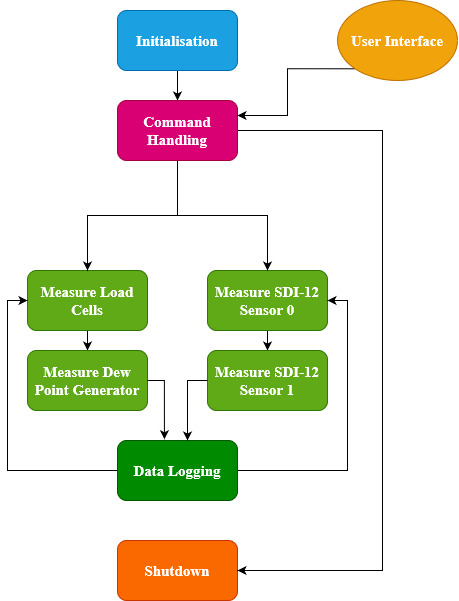
\includegraphics[width=0.4\linewidth]{figures/program_flowchart.jpg}
    \caption{Flowchart of Program}
    \label{flowchart}
\end{figure}

\subsubsection{SDI-12/UART/RS485 Communication}

\textbf{Physical Layer}

SDI-12 communication is managed using UART1 on the RP2040 microcontroller, with specific 
GPIO pins defined for transmission (TX), reception (RX), and data line drive enablement. The SDI-12 protocol operates over a single data line with negative logic levels: logic '0' is high voltage; logic '1' is low voltage. The RS485 transceiver adapts the UART signals to meet these requirements.

The RS485 transceiver is suitable because \cite{AnalogDevicesMAX1487}:

\begin{itemize} 
    \item \textbf{UART Compatibility}: It interfaces easily with UART and supports SDI-12's 1200 baud rate. 
    \item \textbf{Noise Immunity}: Differential signaling enhances noise immunity for reliable long-distance communication. 
    \item \textbf{Line Driving Capability}: Drives long, high-capacitance cables, maintaining signal integrity. 
    \item \textbf{Inverted Logic Handling}: Accommodates the inverted logic levels of SDI-12 devices. 
\end{itemize}

By using only the non-inverting line and proper voltage references, we adapted UART to meet SDI-12's physical layer requirements.

\textbf{Data Link Layer}

The SDI-12 protocol defines communication between the data recorder (master) and sensors (slaves) at 1200 baud, using 7 data bits, even parity, and one stop bit \cite{sdi12_datasheet}. It specifies ASCII commands for initiating measurements, requesting data, and managing sensor addresses \cite{sdi12_datasheet}.

In the current implementation, the system communicates with two SDI-12 sensors with hardcoded addresses. While this simplifies software development, it limits scalability and requires prior knowledge of sensor addresses. SDI-12 supports up to ten sensors on a single data line, each with a unique address \cite{sdi12_datasheet}.

\textbf{Application Layer}

Custom drivers were developed for each sensor, adhering to the SDI-12 protocol. Specific issues with the byte framing of the protocol were addressed by using the 
\code{uart_set_format()} function to configure the communication format correctly, allowing the RP2040 
to receive inverted data without additional circuitry \cite{RaspberryPiPicoSDK}. 
The \code{uart_break()} function sends the required break signal, and \code{uart_read_stuff()} reads sensor responses, which are then parsed to extract data \cite{RaspberryPiPicoSDK}. The timing of the SDI-12 protocol is shown 
in \cref{sdi12_timing}.

\begin{figure}
    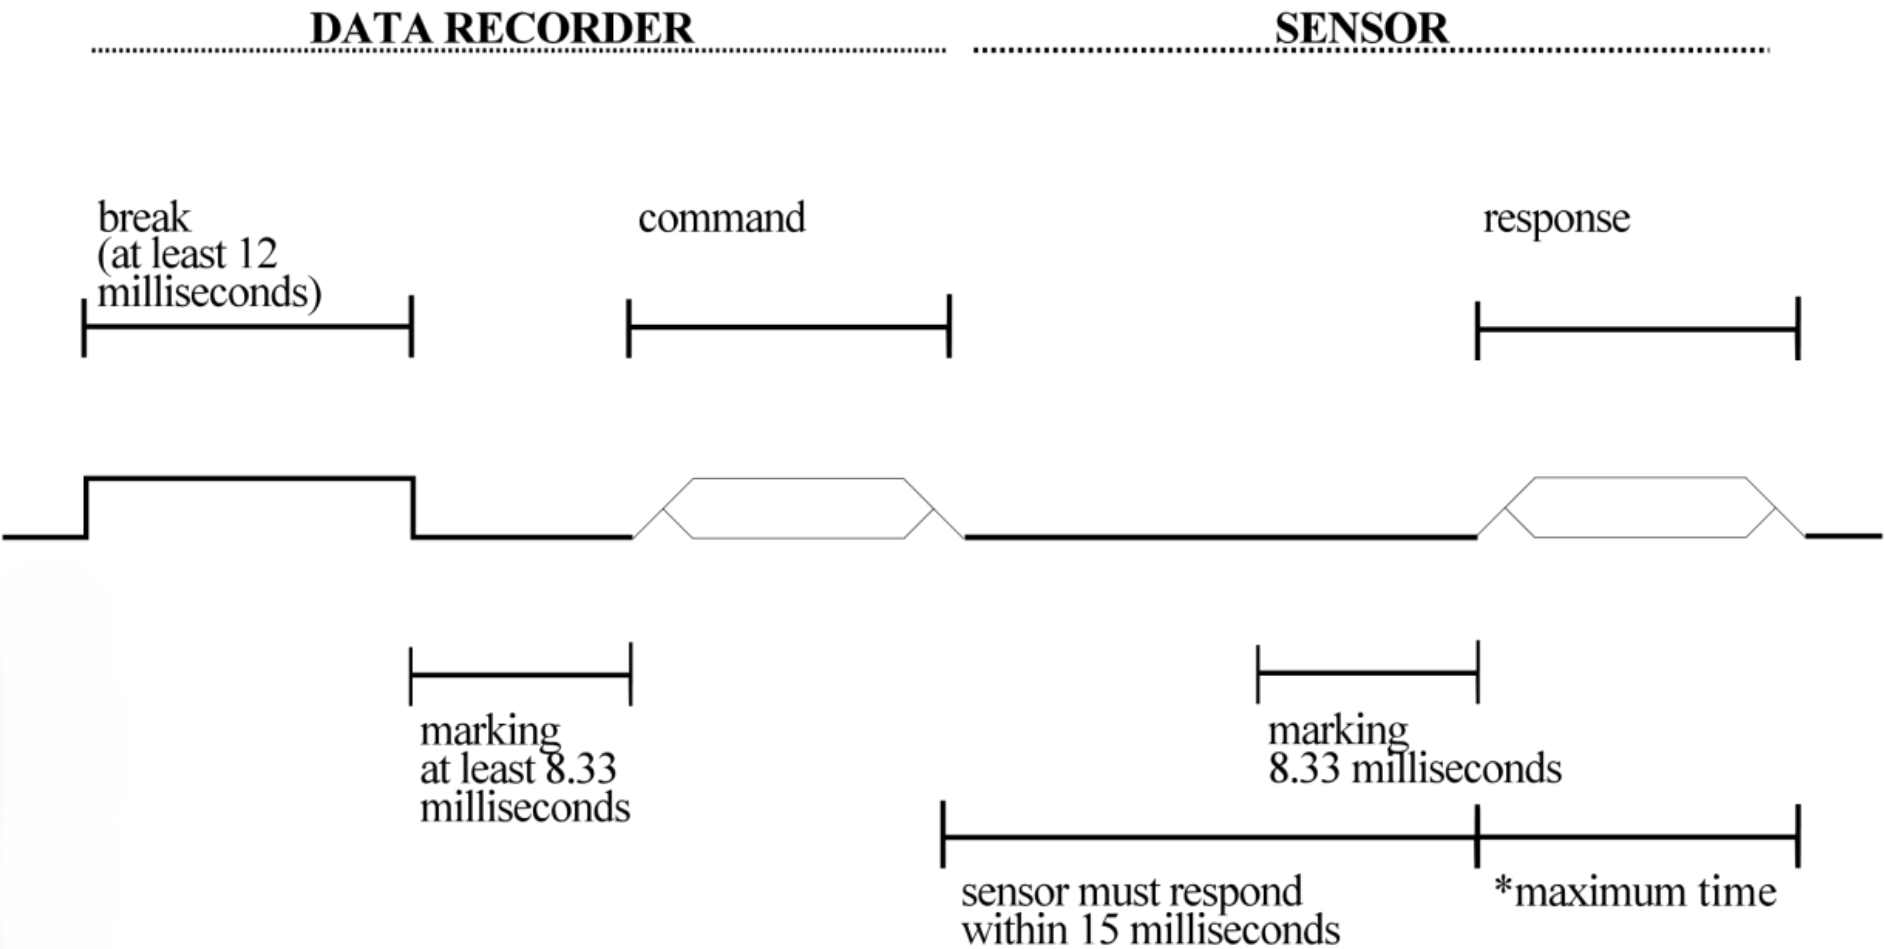
\includegraphics[width=\linewidth]{figures/SDI-12_timing.png}
    \caption{SDI-12 timing from \cite{sdi12_datasheet}}
    \label{sdi12_timing}
\end{figure}

\subsubsection{SPI Communication (SD Card)}

\textbf{Physical Layer}

The SPI protocol is used for communication with the SD card module. SPI is a synchronous serial communication 
interface that operates in full-duplex mode \cite{SPIDevice}. It uses four signals:
\begin{itemize}
    \item MOSI (Master Out Slave In): Transfers data from the master to the slave.
    \item MISO (Master In Slave Out): Transfers data from the slave to the master.
    \item SCK (Serial Clock): Synchronises data transmission between the master and slave.
    \item SS (Slave Select): Enables the slave device for communication.
\end{itemize}
In this system, the SPI bus operates at a clock speed of 1 MHz, suitable for reliable data transfer 
with the SD card.

\textbf{Data Link Layer}

At the data link layer, the SPI protocol exchanges data bytes between the microcontroller 
and the SD card. It does not define a specific frame format or error-checking mechanism, relying on 
higher-level protocols for these functions. The FatFs file system library is employed to handle file 
operations on the SD card. FatFs provides functions for reading, writing, and managing files, ensuring 
data integrity and proper formatting according to the FAT file system standards \cite{NXPMSDFATFSAPI}.

\textbf{Application Layer}

The FatFs API was integrated to enable read/write operations on the SD card, 
using the SPI protocol. This allowed for structured data logging and easy retrieval of information. 
Functions were implemented to write data in CSV format, facilitating compatibility with data analysis tools.

\subsubsection{I2C Communication (DAC)}

\textbf{Physical Layer}

The I2C protocol is used for communication with the MCP4716 DAC. I2C is a synchronous, multi-master, 
multi-slave, single-ended serial communication bus \cite{DAC_datasheet}. It uses two bidirectional open-drain lines:
\begin{itemize}
    \item SDA (Serial Data Line): Transfers data between devices.
    \item SCL (Serial Clock Line): Provides the clock signal for synchronisation.
\end{itemize}
Pull-up resistors are used on both lines to maintain the high logic level when the bus is idle. 
In this system, the I2C bus operates at a standard mode speed of 100 kHz.

\textbf{Data Link Layer}

At the data link layer, the I2C protocol handles addressing and data transfer between the master 
(RP2040 microcontroller) and the slave device (DAC) \cite{DAC_datasheet}. Each device on the I2C bus has a unique 7-bit address. 
The protocol defines start and stop conditions, acknowledgments, and data byte transfers \cite{DAC_datasheet}. The software includes drivers to configure the DAC's settings, such as reference voltage and gain, and to send digital values that the DAC converts into analog voltages. This allows precise control over the dew point generator. These configuartions were all passed on through the \code{Write All Memory} command \cite{DAC_datasheet}.

\subsubsection{Analogue Inputs and Outputs}

\textbf{Physical Layer}

Analog inputs and outputs interface with devices like the load cell (MT-603) and the dew point generator (LI-610). The load cell produces a voltage proportional to the applied weight, connected to the RP2040's ADC pins. An instrumentation amplifier (INA826) amplifies the small signal from the load cell. The dew point generator accepts a 0–5 V analog input for control, provided by the DAC's output.

\textbf{Data Link Layer}

While analog signals lack a formal data link layer, signal conditioning and conversion serve similar functions. For analog inputs, the load cell signal is amplified and filtered before ADC digitization. For analog outputs, the DAC converts digital values into precise voltages to control the dew point generator's settings.

\textbf{Application Layer}

A software interface controls the dew point generator via the I2C protocol communicating with the DAC (MCP4716). This allows precise voltage adjustments, with tests confirming accurate outputs based on command inputs. I2C communication operates in standard mode at 100 kHz, compatible with the DAC \cite{DAC_datasheet}.

Selecting appropriate communication interfaces and voltage levels, along with robust software integration, enables the system to operate seamlessly and efficiently, providing a reliable solution for monitoring and controlling environmental parameters.

